\chapter{Background}
In this chapter we are introducing knowledge which is required to understand the content of this thesis.
In \cref{sec:bg:compilers} we give an overview about how a compiler is typically implemented and which problems it has to solve that we want to tackle.
The \crefrange{sec:bg:compilers:frontend}{sec:bg:compilers:optimizer} give a superficial overview of the first two phases of a typical compiler.
\Cref{sec:bg:compilers:backend} gives a more detailed introduction to compiler back ends, which we aim to optimize in this thesis.
\todo{explain also the other sections}

% NOTE: Assume that the reader has common computer science knowledge!

% --- CPU ---
% Pipeline
% https://de.wikipedia.org/wiki/Pipeline_(Prozessor)
%   - Stages
%   - Hazards
% 
% Skalar - 1 in instruction per cycle possible
% Superskalar - more than 1 instruction per cycle possible
% https://de.wikipedia.org/wiki/Superskalarit%C3%A4t
%   - in order - static
%   - out of order - dynamic
%   - VLIW - multiple commands encoded into one long command

\section{Central Processing Unit}
\label{sec:bg:cpu}
Almost all computer systems use some kind of \acp{cpu}.
It is the main execution unit and executes the vast majority of computer programs on most systems.
It also handles accesses to other parts of the system.
These other parts can be for example the main memory, hard drives, network cards or co-processors like a Graphics Processing Unit.

The \ac{cpu} executes mostly simple instructions, like add, subtract, multiply, shift, or load and store data to/from the main memory.
However, on modern \acp{cpu} there are slightly more complex instructions like combined multiply and add or cryptographic instructions.
The Instruction Set Architecture of a processor architecture defines all of the available instructions of a \ac{cpu}.

Most of the instructions do not have direct access to the main memory.
The instructions typically access data that is stored in the \ac{cpu} registers, which is the fastest memory available.
Hence, before we can execute instructions on some data, we have to transfer this data to the registers.
We transfer the data back to main memory, once we finished out computations.
For example, if we want to compute 
\begin{equation}
    a=a\times a+b\times b+c\times c
    \label{eqn:bg:abc}
\end{equation}
we have to load the data from the variables $a$, $b$, and $c$, make the computations and store the result back to memory.
\Cref{tbl:bg:pipeline-comp-schedule} shows an example implementation in assembly language.
\Cref{fig:bg:example-dag} illustrates the dependencies between the \ac{cpu} instructions of the example implementation.

\begin{table}
    % \scriptsize
    % \lstset{basicstyle=\ttfamily\scriptsize}
    \centering
    \parbox[b][0.93\textheight][s]{0.46\textwidth}{%
        \centering
        \subcaptionbox{Example assembly implementation for \cref{eqn:bg:abc}\label{tbl:bg:pipeline-comp-schedule}}[0.45\textwidth]{%
            \begin{tabular}{rllcl} \toprule
                No.&\multicolumn{4}{c}{Instruction}\\
                \midrule
                1 & \iloccmd{load}{\ilocreg{arp}, @a}{\ilocreg{a}} \\
                2 & \iloccmd{load}{\ilocreg{arp}, @b}{\ilocreg{b}} \\
                3 & \iloccmd{load}{\ilocreg{arp}, @c}{\ilocreg{c}} \\
                4 & \iloccmd{mult}{\ilocreg{a}, \ilocreg{a}}{\ilocreg{a}} \\
                5 & \iloccmd{mult}{\ilocreg{b}, \ilocreg{b}}{\ilocreg{b}} \\
                6 & \iloccmd{mult}{\ilocreg{c}, \ilocreg{c}}{\ilocreg{c}} \\
                7 & \iloccmd{add}{\ilocreg{a}, \ilocreg{b}}{\ilocreg{a}} \\
                8 & \iloccmd{add}{\ilocreg{a}, \ilocreg{c}}{\ilocreg{a}} \\
                9 & \iloccmd{store}{\ilocreg{a}}{\ilocreg{arp}, @a} \\
                \bottomrule
            \end{tabular}
        }
        \vfill
        \subcaptionbox{CPU without pipeline\label{tbl:bg:wo-pipeline}}[0.46\textwidth]{%
            \scriptsize
            \begin{tabular}{rccccccccc} \toprule
                & \multicolumn{9}{c}{\fontsize{11pt}{9pt}\selectfont Instructions (see \cref{tbl:bg:pipeline-comp-schedule})} \\
                \cmidrule{2-10}
                {\fontsize{11pt}{9pt}\selectfont CPU Cycle} & {\fontsize{11pt}{9pt}\selectfont 1} & {\fontsize{11pt}{9pt}\selectfont 2} & {\fontsize{11pt}{9pt}\selectfont 3} & {\fontsize{11pt}{9pt}\selectfont 4} & {\fontsize{11pt}{9pt}\selectfont 5} & {\fontsize{11pt}{9pt}\selectfont 6} & {\fontsize{11pt}{9pt}\selectfont 7} & {\fontsize{11pt}{9pt}\selectfont 8} & {\fontsize{11pt}{9pt}\selectfont 9} \\
                \midrule
                 1 & F &   &   &   &   &   &   &   &   \\ \rowcolor[gray]{.975}
                 2 & D &   &   &   &   &   &   &   &   \\
                 3 & E &   &   &   &   &   &   &   &   \\ \rowcolor[gray]{.975}
                 4 & W &   &   &   &   &   &   &   &   \\
                 5 &   & F &   &   &   &   &   &   &   \\ \rowcolor[gray]{.975}
                 6 &   & D &   &   &   &   &   &   &   \\
                 7 &   & E &   &   &   &   &   &   &   \\ \rowcolor[gray]{.975}
                 8 &   & W &   &   &   &   &   &   &   \\
                 9 &   &   & F &   &   &   &   &   &   \\ \rowcolor[gray]{.975}
                10 &   &   & D &   &   &   &   &   &   \\
                11 &   &   & E &   &   &   &   &   &   \\ \rowcolor[gray]{.975}
                12 &   &   & W &   &   &   &   &   &   \\
                13 &   &   &   & F &   &   &   &   &   \\ \rowcolor[gray]{.975}
                14 &   &   &   & D &   &   &   &   &   \\
                15 &   &   &   & E &   &   &   &   &   \\ \rowcolor[gray]{.975}
                16 &   &   &   & W &   &   &   &   &   \\
                17 &   &   &   &   & F &   &   &   &   \\ \rowcolor[gray]{.975}
                18 &   &   &   &   & D &   &   &   &   \\
                19 &   &   &   &   & E &   &   &   &   \\ \rowcolor[gray]{.975}
                20 &   &   &   &   & W &   &   &   &   \\
                21 &   &   &   &   &   & F &   &   &   \\ \rowcolor[gray]{.975}
                22 &   &   &   &   &   & D &   &   &   \\
                23 &   &   &   &   &   & E &   &   &   \\ \rowcolor[gray]{.975}
                24 &   &   &   &   &   & W &   &   &   \\
                25 &   &   &   &   &   &   & F &   &   \\ \rowcolor[gray]{.975}
                26 &   &   &   &   &   &   & D &   &   \\
                27 &   &   &   &   &   &   & E &   &   \\ \rowcolor[gray]{.975}
                28 &   &   &   &   &   &   & W &   &   \\
                29 &   &   &   &   &   &   &   & F &   \\ \rowcolor[gray]{.975}
                30 &   &   &   &   &   &   &   & D &   \\
                31 &   &   &   &   &   &   &   & E &   \\ \rowcolor[gray]{.975}
                32 &   &   &   &   &   &   &   & W &   \\
                33 &   &   &   &   &   &   &   &   & F \\ \rowcolor[gray]{.975}
                34 &   &   &   &   &   &   &   &   & D \\
                35 &   &   &   &   &   &   &   &   & E \\ \rowcolor[gray]{.975}
                36 &   &   &   &   &   &   &   &   & W \\
                \bottomrule
            \end{tabular}
        }
    }
    \hfill
    \parbox[b][0.93\textheight][s]{0.46\textwidth}{%
        \scriptsize
        \centering
        \subcaptionbox{CPU with scalar pipeline\label{tbl:bg:scalar-pipeline}}[0.46\textwidth]{%
            \begin{tabular}{rccccccccc} \toprule
                & \multicolumn{9}{c}{\fontsize{11pt}{9pt}\selectfont Instructions (see \cref{tbl:bg:pipeline-comp-schedule})} \\
                \cmidrule{2-10}
                {\fontsize{11pt}{9pt}\selectfont CPU Cycle} & {\fontsize{11pt}{9pt}\selectfont 1} & {\fontsize{11pt}{9pt}\selectfont 2} & {\fontsize{11pt}{9pt}\selectfont 3} & {\fontsize{11pt}{9pt}\selectfont 4} & {\fontsize{11pt}{9pt}\selectfont 5} & {\fontsize{11pt}{9pt}\selectfont 6} & {\fontsize{11pt}{9pt}\selectfont 7} & {\fontsize{11pt}{9pt}\selectfont 8} & {\fontsize{11pt}{9pt}\selectfont 9} \\
                \midrule
                 1 & F &   &   &   &   &   &   &   &   \\ \rowcolor[gray]{.975}
                 2 & D & F &   &   &   &   &   &   &   \\
                 3 & E & D & F &   &   &   &   &   &   \\ \rowcolor[gray]{.975}
                 4 & W & E & D &   &   &   &   &   &   \\
                 5 &   & W & E & F &   &   &   &   &   \\ \rowcolor[gray]{.975}
                 6 &   &   & W & D & F &   &   &   &   \\
                 7 &   &   &   & E & D & F &   &   &   \\ \rowcolor[gray]{.975}
                 8 &   &   &   & W & E & D &   &   &   \\
                 9 &   &   &   &   & W & E &   &   &   \\ \rowcolor[gray]{.975}
                10 &   &   &   &   &   & W & F &   &   \\
                11 &   &   &   &   &   &   & D &   &   \\ \rowcolor[gray]{.975}
                12 &   &   &   &   &   &   & E &   &   \\
                13 &   &   &   &   &   &   & W &   &   \\ \rowcolor[gray]{.975}
                14 &   &   &   &   &   &   &   & F &   \\
                15 &   &   &   &   &   &   &   & D &   \\ \rowcolor[gray]{.975}
                16 &   &   &   &   &   &   &   & E &   \\
                17 &   &   &   &   &   &   &   & W &   \\ \rowcolor[gray]{.975}
                18 &   &   &   &   &   &   &   &   & F \\
                19 &   &   &   &   &   &   &   &   & D \\ \rowcolor[gray]{.975}
                20 &   &   &   &   &   &   &   &   & E \\
                21 &   &   &   &   &   &   &   &   & W \\
                \bottomrule
            \end{tabular}
        }
        \vfill
        \subcaptionbox{CPU with superscalar pipeline\label{tbl:bg:superscalar-pipeline}}[0.46\textwidth]{%
            \begin{tabular}{rccccccccc} \toprule
                & \multicolumn{9}{c}{\fontsize{11pt}{9pt}\selectfont Instructions (see \cref{tbl:bg:pipeline-comp-schedule})} \\
                \cmidrule{2-10}
                {\fontsize{11pt}{9pt}\selectfont CPU Cycle} & {\fontsize{11pt}{9pt}\selectfont 1} & {\fontsize{11pt}{9pt}\selectfont 2} & {\fontsize{11pt}{9pt}\selectfont 3} & {\fontsize{11pt}{9pt}\selectfont 4} & {\fontsize{11pt}{9pt}\selectfont 5} & {\fontsize{11pt}{9pt}\selectfont 6} & {\fontsize{11pt}{9pt}\selectfont 7} & {\fontsize{11pt}{9pt}\selectfont 8} & {\fontsize{11pt}{9pt}\selectfont 9} \\
                \midrule
                 1 & F & F &   &   &   &   &   &   &   \\ \rowcolor[gray]{.975}
                 2 & D & D & F &   &   &   &   &   &   \\
                 3 & E & E & D &   &   &   &   &   &   \\ \rowcolor[gray]{.975}
                 4 & W & W & E &   &   &   &   &   &   \\
                 5 &   &   & W & F & F &   &   &   &   \\ \rowcolor[gray]{.975}
                 6 &   &   &   & D & D & F &   &   &   \\
                 7 &   &   &   & E & E & D &   &   &   \\ \rowcolor[gray]{.975}
                 8 &   &   &   & W & W & E &   &   &   \\
                 9 &   &   &   &   &   & W & F &   &   \\ \rowcolor[gray]{.975}
                10 &   &   &   &   &   &   & D &   &   \\
                11 &   &   &   &   &   &   & E &   &   \\ \rowcolor[gray]{.975}
                12 &   &   &   &   &   &   & W &   &   \\
                13 &   &   &   &   &   &   &   & F &   \\ \rowcolor[gray]{.975}
                14 &   &   &   &   &   &   &   & D &   \\
                15 &   &   &   &   &   &   &   & E &   \\ \rowcolor[gray]{.975}
                16 &   &   &   &   &   &   &   & W &   \\
                17 &   &   &   &   &   &   &   &   & F \\ \rowcolor[gray]{.975}
                18 &   &   &   &   &   &   &   &   & D \\
                19 &   &   &   &   &   &   &   &   & E \\ \rowcolor[gray]{.975}
                20 &   &   &   &   &   &   &   &   & W \\ 
                \bottomrule
            \end{tabular}
        }
    }
    \caption[Comparison of CPU pipeline implementations]{Comparison of CPU pipeline implementations for the example in \cref{eqn:bg:abc}}
    \label{tbl:bg:pipeline}
\end{table}

All the assembly code examples is written in the ILOC pseudo-code language~\cite{engineeringcompiler2007}.
Its instructions are of the form \iloccmdinl{instruction}{source}{target}.
The register \ilocreg{arp} is defined to point to the start of a memory block where all variables are saved.
Variables are addressed by adding an offset to the memory address in \ilocreg{arp}.
This is done by adding \eg \iloc{@a} for the variable \iloc{a}.

Instructions that a \ac{cpu} executes are separated into different processing units.
Processing units that typically exist on modern \acp{cpu} are arithmetic logical units, load/store units, floating point units, or encryption units.
These units often exist redundantly on the \acp{cpu}.

\subsection{Classical Instruction Execution}
The execution of instructions is split up into multiple stages.
The number of stages depend on the specific implementation, \eg the ARM Cortex A53 has 8 stages.
A typical example are 4 stages, that usually exist in the most \acp{cpu}.
These stages are:
\begin{enumerate}
    \item Fetch: 
        In this stage, the \ac{cpu} loads the instruction from memory, where the whole program is saved. 
    \item Decode:
        The operands of the instructions are determined.
        The actual memory address will be computed if there are memory addresses with offsets.
    \item Execution:
        Here, the instruction is executed with the given operands on the respective processing unit.
    \item Writeback:
        During this stage, the computed result will be written back to the specified register.
\end{enumerate}

One instruction is executed at a time in this classical execution scheme.
This means that a instruction can only start after all execution stages of the previous instruction have finished.
% Consequently, the throughput of instructions per cycle $t$ is always $t>1$, given that instructions require more than one cycle to execute.

\Cref{tbl:bg:pipeline} compares different execution models for the computation in \cref{eqn:bg:abc} with its implementation in \cref{tbl:bg:pipeline-comp-schedule}.
In this example, we assume that each of the stages Fetch (F), Decode (D), Execution (E) and Writeback (W) take a single \ac{cpu} cycle to finish.
\Cref{tbl:bg:wo-pipeline} shows the execution for this classical execution model.
We see, that the execution takes 36 cycles to finish in this example.

It is easy to see, that the \ac{cpu} stages are not fully utilized.
In fact, only one stage is working at a time and the rest of the stages are doing nothing for the most time.
This is ineffective and is addressed with the next execution model.

\subsection{Scalar Pipeline Execution}
This execution model uses the fact, that most stages are waiting most of the time.
The improvement is that now, one execution can be scheduled every \ac{cpu} cycle.

See in \cref{tbl:bg:scalar-pipeline} that this change introduces parallelism and the first three instruction are executed concurrently.
The theoretically best case is that all the stages are working in every cycle and are never waiting.
This is not always possible, as we can see in the example.
We cannot start instruction 4 (\iloccmdinl{mult}{\ilocreg{a},~\ilocreg{a}}{\ilocreg{a}}) in the \ac{cpu} cycle 4, because we have a dependency on the result of instruction 1 (\iloccmdinl{load}{\ilocreg{arp},~@a}{\ilocreg{a}}).
In cycle 5, the result of instruction 1 was written back and we can start instruction 4.
Different reasons of hazards exist that cause these bubbles in the pipeline.
\begin{itemize}
    \item Ressource Hazards:
        When the \ac{cpu} needs to access a ressource, which is already accessed and thus blocked, the access cannot happen and has to wait.
        This could, for example, happen with registers that have only one access line.
        Redundancy of hardware units can solve or mitigate this problem.
    \item Data Hazards:
        Three types of different data hazards exist when two instructions want to access the same register:
        \begin{itemize}
            \item Read after write: A instruction has to wait until a previous instruction has produced the result that the latter has to read.
            \item Write after read: A instruction has to wait until a previous instruction has read a register, that the latter has to overwrite.
            \item Write after write: A instruction has to wait until a previous instruction has written a register, that the latter wants to write to, too.
        \end{itemize}
        These hazards are typically solved by sorting the instructions or when its unavoidable by waiting and introducing bubbles into the pipeline.
    \item Control Hazards:
        It is not always obvious which instruction should be executed next due to if/else constructs or loops.
        Usually, one branch will be speculatively executed and the instructions will be aborted if it was the wrong branch.
        This problem is typically approached by branch prediction mechanisms that can be done in the compiler and also on the hardware.
\end{itemize}

\subsection{Superscalar Pipeline Execution}
The next progression from the scalar pipeline is this pipeline model.
The difference is, that we can start multiple instructions in the same \ac{cpu} cycle.
Consequently, the level parallelism is further increased.
The number of instructions that can be started simultaneously depends on the specific hardware. % A53 2-way

\Cref{tbl:bg:superscalar-pipeline} shows an example execution of a two way superscalar pipeline.
This is especially interesting to compare with the scalar pipeline in \cref{tbl:bg:scalar-pipeline}.
Note, that now, the instructions 1 and 2 are scheduled in the same \ac{cpu} cycle.
If we had simulated a three way superscalar pipeline, we could have started instructions 1-3 in the first cycle.
However, we still have a runtime improvement of one cycle compared to the scalar pipeline.

Superscalar pipelines can be implemented in various ways.
The three most typical implementations are:
\begin{itemize}
    \item In order (static): 
        These type of \acp{cpu} take the instructions as they come and check if they can be executed simultaneously.
        The instruction schedule is defined by the compiler.
    \item Out of order (dynamic): 
        Contrarily, dynamic superscalar \acp{cpu} are able to see the next $n$ instructions and can reschedule them, such that a higher parallelism is achieved.
        This means that the compiler does not has full control on the executed instruction schedule, which is a important aspect for this thesis.
    \item Very Long Instruction Word: 
        For this type of superscalar pipeline, the compiler can define which instructions the \ac{cpu} will execute simultaneously.
        This assignment works by wrapping multiple instructions into a single instruction, thus the name.
\end{itemize}

\begin{figure}
    \centering

    % TODO: move these definitions somewhere else?
    \definecolor{darkgray}{HTML}{3D4752}
    \tikzstyle{instr} = [rectangle, rounded corners, minimum width=3cm, minimum height=1cm,text centered, text=white, fill=darkgray]
    \tikzstyle{arrow} = [thick,->,>=stealth]
    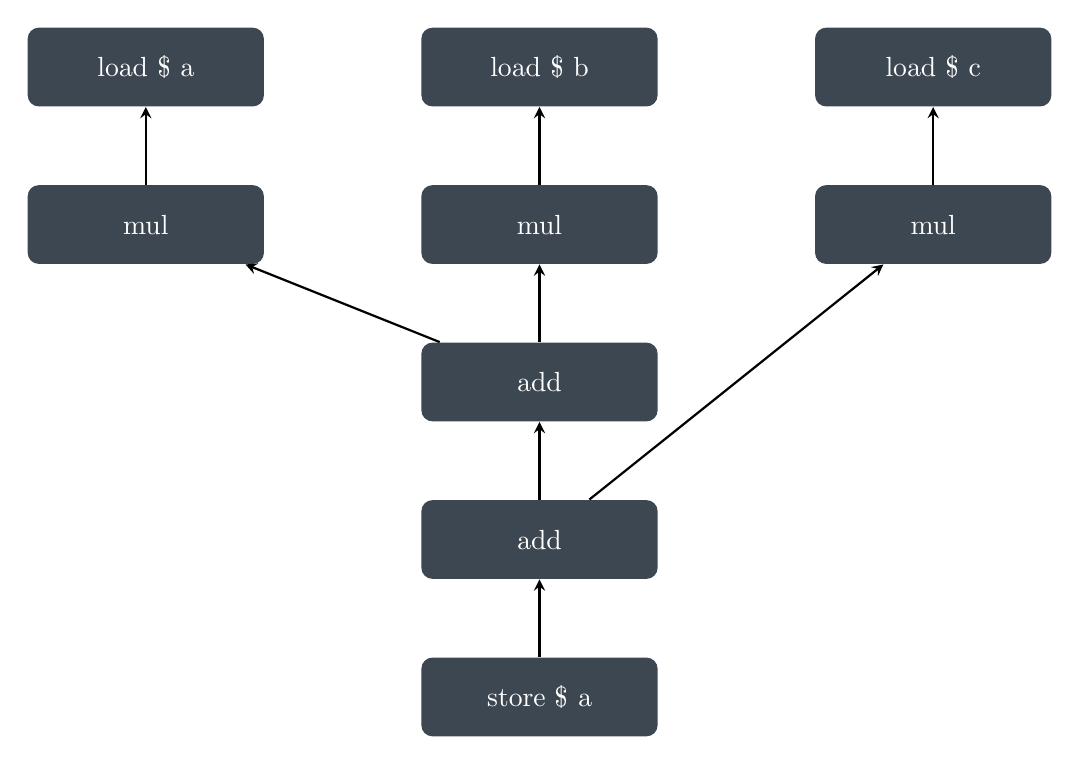
\begin{tikzpicture}[node distance=2cm]
        \node (load_a) [instr] {\lstinline{load \$ a}};
        \node (mul_a_a) [instr, below of=load_a] {\lstinline{mul}};
        \node (load_b) [instr, right of=load_a, xshift=3cm] {\lstinline{load \$ b}};
        \node (mul_b_b) [instr, below of=load_b] {\lstinline{mul}};
        \node (load_c) [instr, right of=load_b, xshift=3cm] {\lstinline{load \$ c}};
        \node (mul_c_c) [instr, below of=load_c] {\lstinline{mul}};
        \node (add_a_b) [instr, below of=mul_b_b] {\lstinline{add}};
        \node (add_ab_c) [instr, below of=add_a_b] {\lstinline{add}};
        \node (store) [instr, below of=add_ab_c] {\lstinline{store \$ a}};
        
        \draw [arrow] (mul_a_a) -- (load_a);
        \draw [arrow] (mul_b_b) -- (load_b);
        \draw [arrow] (mul_c_c) -- (load_c);
        \draw [arrow] (add_a_b) -- (mul_a_a);
        \draw [arrow] (add_a_b) -- (mul_b_b);
        \draw [arrow] (add_ab_c) -- (add_a_b);
        \draw [arrow] (add_ab_c) -- (mul_c_c);
        \draw [arrow] (store) -- (add_ab_c);    
    \end{tikzpicture}
    \caption{Example DAG a=a*a+b*b+c*c}
    \label{fig:bg:example-dag}
\end{figure}

% \begin{table}
%     \centering
%     \begin{tabular}{cclcl} 
%         \toprule
%         Start & Occupied & \multicolumn{3}{l}{Instruction} \\
%         Cycle &  Cycles &&&\\
%         \midrule
%         1  & 1-3   & \lstinline{load \$ a}  & \rightarrow & \lstinline{a} \\
%         4  & 4-5   & \lstinline{mul a, a} & \rightarrow & \lstinline{a} \\
%         5  & 5-7   & \lstinline{load \$ b}  & \rightarrow & \lstinline{b} \\
%         8  & 8-9   & \lstinline{mul b, b} & \rightarrow & \lstinline{b} \\
%         9  & 9-11  & \lstinline{load \$ c}  & \rightarrow & \lstinline{c} \\
%         12 & 12-13 & \lstinline{mul c, c} & \rightarrow & \lstinline{c} \\
%         13 & 13    & \lstinline{add a, b} & \rightarrow & \lstinline{a} \\
%         14 & 14    & \lstinline{add a, c} & \rightarrow & \lstinline{a} \\
%         15 & 15-17 & \lstinline{store a}  & \rightarrow & \lstinline{\$ a} \\
%         \bottomrule
%     \end{tabular}
%     \caption{Unscheduled example \lstinline{a=a*a+b*b+c*c}}
%     \label{table:1}
% \end{table}

% \begin{table}
%     \centering
%     \begin{tabular}{cclcl} 
%         \toprule
%         Start & Occupied & \multicolumn{3}{l}{Instruction} \\
%         Cycle &  Cycles &&&\\
%         \midrule
%         1 & 1-3  & \lstinline{load \$ a}  & \rightarrow & \lstinline{a} \\
%         2 & 2-4  & \lstinline{load \$ b}  & \rightarrow & \lstinline{b} \\
%         3 & 3-5  & \lstinline{load \$ c}  & \rightarrow & \lstinline{c} \\
%         4 & 4-5  & \lstinline{mul a, a} & \rightarrow & \lstinline{a} \\
%         5 & 5-6  & \lstinline{mul b, b} & \rightarrow & \lstinline{b} \\
%         6 & 6-7  & \lstinline{mul c, c} & \rightarrow & \lstinline{c} \\
%         7 & 7    & \lstinline{add a, b} & \rightarrow & \lstinline{a} \\
%         8 & 8    & \lstinline{add a, c} & \rightarrow & \lstinline{a} \\
%         9 & 9-11 & \lstinline{store a}  & \rightarrow & \lstinline{\$ a} \\
%         \bottomrule
%     \end{tabular}
%     \caption{Scheduled example \lstinline{a=a*a+b*b+c*c}}
%     \label{table:2}
% \end{table}

\section{Compilers}
\label{sec:bg:compilers}
%What is a compiler? \\
% \todo{This is probably too basic and not required. Might maybe be used in introduction, though}
% In the early days of computer programming, computers were programmed in assembly languages.
% These languages are exclusive to specific processor architectures and only provide the instructions that are available by the \ac{isa} of the processor.
% This approach has several disadvantages.
% Lots of complicated code, that is hard to understand, is written to express even simple programs.
% Also, each program has to be rewritten to execute on a processor with another architecture.
%
% Nowadays computers are programmed---almost exclusively---in high-level programming languages like C/C++, Java, Python, etc.
% The processor is not able to execute code written in such high-level programming languages, though.
% For this reason a compiler has to translate the code into a format that the processor can understand.
Making computer programs, that are written in high-level programming languages~(\eg C/C++, Java, Rust), executable on a specific machine is not a trivial task.
Compilers are only one piece in the tool-chain required to make a program executable.
The compiler translates the high-level language into assembly language, which is translated into object code by the assembler.
Basic functionality like allocating memory or outputting strings on the screen is implemented in a standard library.
The object code of the standard library and potentially other libraries are linked together with the translated program by the linker.
There is more required to execute the code on a specific machine (\eg a runtime library), but explaining this would go beyond the scope of this thesis.

%Why are compilers important? \\
%What are the different tasks a compiler has? \\
The pure translation of the program is only one of the tasks a compiler has to fulfill.
It also has to assure that the program is written in correct syntax of the high-level language.
Most compilers will also optimize the given code and the translated code since a simple one-to-one translation would have a very poor performance.
Eventually there has to be a mapping from variables and to the main memory and the processors registers.
These are all by itself complex problems which are handled by a compiler.

%How are compilers usually implemented? (Front-End, ...)\\
Compilers are usually implemented in different phases to seperate the different tasks and have a structured approach.
A common approach to structure a compiler is by having a front end~(\cref{sec:bg:compilers:frontend}), an optional optimization~(\cref{sec:bg:compilers:optimizer}) and a back end phase~(\cref{sec:bg:compilers:backend}).
These phases are explained in more detail in the following sub sections.

\subsection{Front End}
\label{sec:bg:compilers:frontend}
The front end phase is the first step in the translation process.
Its implementation is dependent on the source language that has to be translated.
A typical front end includes a scanner, a syntax checker/parser, a context-sensitive analysis and translation into a \ac{ir}.
The scanner translates a stream of characters into a stream of tokens that are classified as parts of the source language.
These tokens are then taken by the parser and are checked against the grammer defined by the source language.
Even with a syntactically correct program, there can still be errors in the code, \eg assignments of incompatible types.
These are checked during the context-sensitive analysis phase.
Eventually, the source code is translated into some kind of a \ac{ir} which will be used as input to the optimizer and the back end.

There might be additional steps required depending on the source language.
C/C++ compilers, for example, use a preprocessor to replace macros like \lstinline[language=C]{#include} and \lstinline[language=C]{#define} with their actual values.

\subsection{Optimizer}
\label{sec:bg:compilers:optimizer}
The usage of a \ac{ir}, not only abstracts away the source language and the target hardware, but also permits to apply more passes in the compilation process.
These addition passes transform \ac{ir} to \ac{ir}.
Note that this step is optional and not required to produce correct translations.
The purpose of this step is to optimize the code, in a source and target independent manner, for more efficient execution.
Efficient can mean different things here. % \eg faster, lower memory usage, lower energy consumption.
The transformed code might produce, \eg a faster program, a program that is smaller in size, or a program with less power consumption.
There exist a large amount of optimization passes in most compilers.
They range from rather simple optimizations, like replacing constant variables with their actual value, to more advanced ones that might, for example, simpliy computations with the rules of algebra.

\subsection{Back End}
\label{sec:bg:compilers:backend}
The compilers back end takes the \ac{ir} as input and emits code for the target hardware and decides which variables will reside in registers only and which ones reside in memory.
This last step consists of three main tasks.

The first step is the instruction selection.
Instruction selection translates the operations of the \ac{ir} to operations of the \ac{isa} of the target hardware.
The next steps, instruction scheduling and register allocation are explained in a little more detail as they represent the main topic of this thesis.

\subsubsection{Instruction Scheduling}
%\section{Motivation?}
%\cite{goodman1988code} state the important interdependence between instruction scheduling and register allocation.
Add Example: e.g. see \url{https://youtu.be/brpomKUynEA?t=271} \\
Probably best to introduce an example in the \cref{sec:bg:cpu} and reuse/extend it here.
Typically works on Basic Blocks. What is a Basic Block?

\subsubsection{Register Allocation}
The usage of an infinite amount of virtual registers in the \ac{ir} was ignored in the instruction selection step.

\section{LLVM Compiler Infrastructure}
\subsection{Intermediate Representation}
\subsection{Instruction Selection DAG}
\begin{figure}
    \centering
    \includegraphics[width=\textwidth]{img/example-dag-crop.pdf}
    \caption[Example \aclu{dag} generated by LLVM]{Example \ac{dag} generated by LLVM. It shows the (AARCH64) instructions defined by LLVM and the dependencies between the instructions.}
    \label{fig:bg:dag}
\end{figure}
\subsection{Pre-RA-Scheduling}
Welche gibt es?\\
Wie funktionieren sie?\\
Welche Infos nutzen sie?\\
\subsection{Post-RA-Scheduling}

\section{Data-Driven Methods}
\subsection{Reinforcement Learning}
\subsection{Monte Carlo Tree Search}
\label{sec:bg:mcts}
\subsection{Support Vector Machines}
\subsection{Neural Networks}
